\documentclass[11pt]{article}%,twocolumn
\usepackage{url}
\usepackage{cite}
\usepackage{graphicx}
\usepackage{listings}
\usepackage{colortbl}
\usepackage{fancyvrb}
\usepackage{color}
\usepackage[ascii]{inputenc}
\usepackage{titling}
\newcommand{\subtitle}[1]{%
  \posttitle{%
    \par\end{center}
    \begin{center}\large#1\end{center}
    \vskip0.5em}%
}

%\usepackage{appendix}

\makeatletter
\def\PY@reset{\let\PY@it=\relax \let\PY@bf=\relax%
    \let\PY@ul=\relax \let\PY@tc=\relax%
    \let\PY@bc=\relax \let\PY@ff=\relax}
\def\PY@tok#1{\csname PY@tok@#1\endcsname}
\def\PY@toks#1+{\ifx\relax#1\empty\else%
    \PY@tok{#1}\expandafter\PY@toks\fi}
\def\PY@do#1{\PY@bc{\PY@tc{\PY@ul{%
    \PY@it{\PY@bf{\PY@ff{#1}}}}}}}
\def\PY#1#2{\PY@reset\PY@toks#1+\relax+\PY@do{#2}}

\expandafter\def\csname PY@tok@gd\endcsname{\def\PY@tc##1{\textcolor[rgb]{0.63,0.00,0.00}{##1}}}
\expandafter\def\csname PY@tok@gu\endcsname{\let\PY@bf=\textbf\def\PY@tc##1{\textcolor[rgb]{0.50,0.00,0.50}{##1}}}
\expandafter\def\csname PY@tok@gt\endcsname{\def\PY@tc##1{\textcolor[rgb]{0.00,0.27,0.87}{##1}}}
\expandafter\def\csname PY@tok@gs\endcsname{\let\PY@bf=\textbf}
\expandafter\def\csname PY@tok@gr\endcsname{\def\PY@tc##1{\textcolor[rgb]{1.00,0.00,0.00}{##1}}}
\expandafter\def\csname PY@tok@cm\endcsname{\let\PY@it=\textit\def\PY@tc##1{\textcolor[rgb]{0.25,0.50,0.50}{##1}}}
\expandafter\def\csname PY@tok@vg\endcsname{\def\PY@tc##1{\textcolor[rgb]{0.10,0.09,0.49}{##1}}}
\expandafter\def\csname PY@tok@m\endcsname{\def\PY@tc##1{\textcolor[rgb]{0.40,0.40,0.40}{##1}}}
\expandafter\def\csname PY@tok@mh\endcsname{\def\PY@tc##1{\textcolor[rgb]{0.40,0.40,0.40}{##1}}}
\expandafter\def\csname PY@tok@go\endcsname{\def\PY@tc##1{\textcolor[rgb]{0.53,0.53,0.53}{##1}}}
\expandafter\def\csname PY@tok@ge\endcsname{\let\PY@it=\textit}
\expandafter\def\csname PY@tok@vc\endcsname{\def\PY@tc##1{\textcolor[rgb]{0.10,0.09,0.49}{##1}}}
\expandafter\def\csname PY@tok@il\endcsname{\def\PY@tc##1{\textcolor[rgb]{0.40,0.40,0.40}{##1}}}
\expandafter\def\csname PY@tok@cs\endcsname{\let\PY@it=\textit\def\PY@tc##1{\textcolor[rgb]{0.25,0.50,0.50}{##1}}}
\expandafter\def\csname PY@tok@cp\endcsname{\def\PY@tc##1{\textcolor[rgb]{0.74,0.48,0.00}{##1}}}
\expandafter\def\csname PY@tok@gi\endcsname{\def\PY@tc##1{\textcolor[rgb]{0.00,0.63,0.00}{##1}}}
\expandafter\def\csname PY@tok@gh\endcsname{\let\PY@bf=\textbf\def\PY@tc##1{\textcolor[rgb]{0.00,0.00,0.50}{##1}}}
\expandafter\def\csname PY@tok@ni\endcsname{\let\PY@bf=\textbf\def\PY@tc##1{\textcolor[rgb]{0.60,0.60,0.60}{##1}}}
\expandafter\def\csname PY@tok@nl\endcsname{\def\PY@tc##1{\textcolor[rgb]{0.63,0.63,0.00}{##1}}}
\expandafter\def\csname PY@tok@nn\endcsname{\let\PY@bf=\textbf\def\PY@tc##1{\textcolor[rgb]{0.00,0.00,1.00}{##1}}}
\expandafter\def\csname PY@tok@no\endcsname{\def\PY@tc##1{\textcolor[rgb]{0.53,0.00,0.00}{##1}}}
\expandafter\def\csname PY@tok@na\endcsname{\def\PY@tc##1{\textcolor[rgb]{0.49,0.56,0.16}{##1}}}
\expandafter\def\csname PY@tok@nb\endcsname{\def\PY@tc##1{\textcolor[rgb]{0.00,0.50,0.00}{##1}}}
\expandafter\def\csname PY@tok@nc\endcsname{\let\PY@bf=\textbf\def\PY@tc##1{\textcolor[rgb]{0.00,0.00,1.00}{##1}}}
\expandafter\def\csname PY@tok@nd\endcsname{\def\PY@tc##1{\textcolor[rgb]{0.67,0.13,1.00}{##1}}}
\expandafter\def\csname PY@tok@ne\endcsname{\let\PY@bf=\textbf\def\PY@tc##1{\textcolor[rgb]{0.82,0.25,0.23}{##1}}}
\expandafter\def\csname PY@tok@nf\endcsname{\def\PY@tc##1{\textcolor[rgb]{0.00,0.00,1.00}{##1}}}
\expandafter\def\csname PY@tok@si\endcsname{\let\PY@bf=\textbf\def\PY@tc##1{\textcolor[rgb]{0.73,0.40,0.53}{##1}}}
\expandafter\def\csname PY@tok@s2\endcsname{\def\PY@tc##1{\textcolor[rgb]{0.73,0.13,0.13}{##1}}}
\expandafter\def\csname PY@tok@vi\endcsname{\def\PY@tc##1{\textcolor[rgb]{0.10,0.09,0.49}{##1}}}
\expandafter\def\csname PY@tok@nt\endcsname{\let\PY@bf=\textbf\def\PY@tc##1{\textcolor[rgb]{0.00,0.50,0.00}{##1}}}
\expandafter\def\csname PY@tok@nv\endcsname{\def\PY@tc##1{\textcolor[rgb]{0.10,0.09,0.49}{##1}}}
\expandafter\def\csname PY@tok@s1\endcsname{\def\PY@tc##1{\textcolor[rgb]{0.73,0.13,0.13}{##1}}}
\expandafter\def\csname PY@tok@sh\endcsname{\def\PY@tc##1{\textcolor[rgb]{0.73,0.13,0.13}{##1}}}
\expandafter\def\csname PY@tok@sc\endcsname{\def\PY@tc##1{\textcolor[rgb]{0.73,0.13,0.13}{##1}}}
\expandafter\def\csname PY@tok@sx\endcsname{\def\PY@tc##1{\textcolor[rgb]{0.00,0.50,0.00}{##1}}}
\expandafter\def\csname PY@tok@bp\endcsname{\def\PY@tc##1{\textcolor[rgb]{0.00,0.50,0.00}{##1}}}
\expandafter\def\csname PY@tok@c1\endcsname{\let\PY@it=\textit\def\PY@tc##1{\textcolor[rgb]{0.25,0.50,0.50}{##1}}}
\expandafter\def\csname PY@tok@kc\endcsname{\let\PY@bf=\textbf\def\PY@tc##1{\textcolor[rgb]{0.00,0.50,0.00}{##1}}}
\expandafter\def\csname PY@tok@c\endcsname{\let\PY@it=\textit\def\PY@tc##1{\textcolor[rgb]{0.25,0.50,0.50}{##1}}}
\expandafter\def\csname PY@tok@mf\endcsname{\def\PY@tc##1{\textcolor[rgb]{0.40,0.40,0.40}{##1}}}
\expandafter\def\csname PY@tok@err\endcsname{\def\PY@bc##1{\setlength{\fboxsep}{0pt}\fcolorbox[rgb]{1.00,0.00,0.00}{1,1,1}{\strut ##1}}}
\expandafter\def\csname PY@tok@kd\endcsname{\let\PY@bf=\textbf\def\PY@tc##1{\textcolor[rgb]{0.00,0.50,0.00}{##1}}}
\expandafter\def\csname PY@tok@ss\endcsname{\def\PY@tc##1{\textcolor[rgb]{0.10,0.09,0.49}{##1}}}
\expandafter\def\csname PY@tok@sr\endcsname{\def\PY@tc##1{\textcolor[rgb]{0.73,0.40,0.53}{##1}}}
\expandafter\def\csname PY@tok@mo\endcsname{\def\PY@tc##1{\textcolor[rgb]{0.40,0.40,0.40}{##1}}}
\expandafter\def\csname PY@tok@kn\endcsname{\let\PY@bf=\textbf\def\PY@tc##1{\textcolor[rgb]{0.00,0.50,0.00}{##1}}}
\expandafter\def\csname PY@tok@mi\endcsname{\def\PY@tc##1{\textcolor[rgb]{0.40,0.40,0.40}{##1}}}
\expandafter\def\csname PY@tok@gp\endcsname{\let\PY@bf=\textbf\def\PY@tc##1{\textcolor[rgb]{0.00,0.00,0.50}{##1}}}
\expandafter\def\csname PY@tok@o\endcsname{\def\PY@tc##1{\textcolor[rgb]{0.40,0.40,0.40}{##1}}}
\expandafter\def\csname PY@tok@kr\endcsname{\let\PY@bf=\textbf\def\PY@tc##1{\textcolor[rgb]{0.00,0.50,0.00}{##1}}}
\expandafter\def\csname PY@tok@s\endcsname{\def\PY@tc##1{\textcolor[rgb]{0.73,0.13,0.13}{##1}}}
\expandafter\def\csname PY@tok@kp\endcsname{\def\PY@tc##1{\textcolor[rgb]{0.00,0.50,0.00}{##1}}}
\expandafter\def\csname PY@tok@w\endcsname{\def\PY@tc##1{\textcolor[rgb]{0.73,0.73,0.73}{##1}}}
\expandafter\def\csname PY@tok@kt\endcsname{\def\PY@tc##1{\textcolor[rgb]{0.69,0.00,0.25}{##1}}}
\expandafter\def\csname PY@tok@ow\endcsname{\let\PY@bf=\textbf\def\PY@tc##1{\textcolor[rgb]{0.67,0.13,1.00}{##1}}}
\expandafter\def\csname PY@tok@sb\endcsname{\def\PY@tc##1{\textcolor[rgb]{0.73,0.13,0.13}{##1}}}
\expandafter\def\csname PY@tok@k\endcsname{\let\PY@bf=\textbf\def\PY@tc##1{\textcolor[rgb]{0.00,0.50,0.00}{##1}}}
\expandafter\def\csname PY@tok@se\endcsname{\let\PY@bf=\textbf\def\PY@tc##1{\textcolor[rgb]{0.73,0.40,0.13}{##1}}}
\expandafter\def\csname PY@tok@sd\endcsname{\let\PY@it=\textit\def\PY@tc##1{\textcolor[rgb]{0.73,0.13,0.13}{##1}}}

\def\PYZbs{\char`\\}
\def\PYZus{\char`\_}
\def\PYZob{\char`\{}
\def\PYZcb{\char`\}}
\def\PYZca{\char`\^}
\def\PYZam{\char`\&}
\def\PYZlt{\char`\<}
\def\PYZgt{\char`\>}
\def\PYZsh{\char`\#}
\def\PYZpc{\char`\%}
\def\PYZdl{\char`\$}
\def\PYZhy{\char`\-}
\def\PYZsq{\char`\'}
\def\PYZdq{\char`\"}
\def\PYZti{\char`\~}
% for compatibility with earlier versions
\def\PYZat{@}
\def\PYZlb{[}
\def\PYZrb{]}
\makeatother

\pretitle{\begin{center}Master Thesis\\Preparation Report\end{center}\vspace*{15 mm}\begin{center}}

\posttitle{\end{center}\begin{center}\end{center}}

\begin{document}

\title{\huge Towards The Reactive Web\vspace*{15 mm}}
%\subtitle{Master Thesis\\Preparation Report}
\date{\today}
%\author{Dominic Bosch \\ Departement Mathematics and Computer Science \\ University of Basel}
\author{\fontsize{11}{9}\selectfont Dominic Bosch \\ Departement Mathematics and Computer Science \\ University of Basel}
\maketitle

\renewcommand{\abstractname}{}
\begin{abstract}
\textbf{Abstract.}
While identifying related work, it became clear that huge efforts in the research fields of event-driven architectures and user-driven mashup development has been done. On the other hand cloud application utilization is a most recent research field and continues to be a big challenge as they evolve. Moreover the use of cloud applications seems to be a nice feature, rather than founding the basis of research. To the best of our knowledge, no related work was found which funnels all these research fields into one, providing novel powerful ways to govern the web.
\end{abstract}

\section{Introduction}
%The web continuously evolves into bigger complexity, allowing for ever more powerful applications.
In today's large, powerful and dynamic web, the big challenge is to retain manageable interactions between cloud applications, while adopting reactivity to them. To get a hold on this, we are tempting the next change in the evolution of the web: the live web, or reactive web. By considering cloud applications as event producers and action consumers we are able to apply a new level of abstraction to the web, which allows new perspectives and approaches to manifest the reactive web. Such architecture has the potential to overcome limitations that have been encountered during previous research.
%The web over time changed its role. In the first stage, it was a passive document storage driven in client-server mode. Using web 2.0 technology in the next phase more and more desk top computer usage went into the web. Today web clouds are proliferating. We anticipate a next change in the near future: The live web or reactive web.
%The goal of this project is to enhance the web with rule-based event-condition-action (ECA) mechanisms  such that the web turns itself into an reactive entity. After an analysis of current approaches, a generalized ECA language together with a rule engine should be provided. For test and demonstration purposes, usage scenarios should be specified and new web services should be derived. As a case study, the rule engine should be integrated with the ProBinder~\cite{wwwprobinder} software, which is an advanced collaboration platform based on the shelf, binder, and register notion.

\section{Related Work}
\subsection{Reactivity in the Web}
Research approaches to apply reactivity to the web has been done by several researchers in many fields.
%It is often referenced and served as a basis to many future research in terms of reactivity in the web.
In ~\cite{2009-Paschke_Boley-RCER.pdf} the authors provide an overview of general descriptions and classifications from different research efforts in terms of events, rules and reactiveness. The different research domains they point out are:
 \begin{itemize}
%\itemsep-1.5em
  \item Event/Action Logics, Transition Logics and Process Calculi. Used in \cite{Behrends:2008:EEA:1377798.1377801} to specify complex actions
  \item Dynamic/Update/Transition Logics
  \item Production Rule Systems (if-do)
  \item Active Databases and ECA Rule Systems (on-if-do)
  \item Rule-Based Complex Event Processing (CEP) and Event Notification Systems
\end{itemize}
In contrast to standard ECA rules, which typically only have one global state, messaging reaction rules maintain a local conversation state that reflects the process execution state. This supports the performing of different activities within process instances managed in simultaneous conversation branches. Today, powerful event languages (such as \emph{RuleML}) exist, which allow to express each of the afore mentioned categories.

In \cite{2012-Giurca_etal-RuleTheWeb.pdf} semantic application vocabulary and business rules are examined, which together allow smart suggestions to the user in a rule-based system. Their approach bases on Distributed Object Model (DOM) interactions and mashups would have to be constructed indirectly via the DOM. Their work is interesting when allowing the users to customize their online context but it doesn't allow for cloud applications to be first-class citizens as part of on- and offline mashups.

From \cite{2010-Ye_Jacobsen-EEWS.pdf} follows, that enhancing a Service oriented Architecture (SOA) with an event-driven SOA (EDSOA), leads to more flexible and adaptive SOA applications that can be informed about states of neighbouring components. In their approach, events are only an aid to react on unexpected behaviour. But our research path leads us towards a system which builds entirely on events, using their expressive power as a basis.

\subsection{Rules Languages}
%\begin{lstlisting}[breaklines]
%<Rule>
%  [...]
%  <on>      </on>
%   <if>      </if>
%   <then>    </then>
%   <do>      </do>
%   <after>   </after>
%   <else>    </else>
%   <elsedo>  </elsedo>
% </Rule>
% \end{lstlisting}
En excerpt of rule engines and languages is shortly introduced here. The recent trend seems to go towards funneling the different event-based approaches into CEP as highly expressive paradigm to incorporate all others. Of course more rule engines or languages exist, but they either go into similar categories as the presented ones, aren't developed anymore, or haven't been identified in related work as recent or active research.

\subsubsection{XChange/Xcerpt}
One notable outcome of research in the last decade is the language \emph{XChange}~\cite{2005-Patranjan-TLE.pdf,2005-Bry_etal-XChange.pdf}, which introduces reactivity to the web. \emph{XChange} uses \emph{Xcerpt}~\cite{2004-Schaffert-Xcerpt.pdf}, a rule-based query and transformation Language for the web, to express web queries.
\emph{XChange} was part of the REWERSE research project, funded by the EU and Switzerland and is discontinued since 2008. But the paradigms provided by both XChange and Xcerpt found their way into virtually every further research that was later done in the field of reactivity in the web. It mainly influenced both \emph{RuleML} and \emph{JSON Rules} and through this the whole field. 

\subsubsection{JSON Rules}
\emph{JSON Rules}~\cite{2008-Giurca_Pascalau-JSON_Rules.pdf} has been invented due to an increasing need for rules in terms of semantic web applications and the emerging Rich Internet Applications (RIAs). \emph{JSON Rules} is capable of expressing production rules (if-do) as well as ECA rules (on-if-do). The rules engine is a forward chaining rule engine using a modified RETE~\cite{1982-Crockford-RETE.pdf} algorithm. The RETE working memory in this rule engine is the (event-based) Document Object Model (DOM) itself. An example~\cite{2009-Pascalau_Giurca-RBACEM.pdf} of (DOM-)rule-based creation and execution of mashups illustrates the powerful aspects of \emph{JSON Rules}. The current limitation to the DOM tree would require a generalization to adopt it also to other memory layouts. The development of the \emph{JSON Rules} engine is discontinued.


\subsubsection{(Reaction) RuleML}
\textit{RuleML}~\cite{2006-Boley-RuleML.pdf} is a XML-based rule specification standard to express both forward and backward rules for derivation, reaction, rewriting, messaging, verification and transformation. The building blocks of \textit{RuleML} are predicates, derivation rules, facts, queries, integrity constraints and transformation rules. Its development is driven by the Rule Markup Initiative~\cite{wwwruleml}.

With \textit{RuleML} being already a useful specification, \textit{Reaction RuleML}~\cite{2012-Paschke_etal-ReactionRuleML.pdf} extends \textit{RuleML} towards reaction rules and complex event/action messages, e.g. for CEP. It adds various kinds of production, action, reaction and knowledge representation (KR) temporal/event/action logic rules, as well as (complex) event/action messages. It consists of one general reaction rule form that can be specialized, e.g. into production rules, trigger rules, ECA rules or messaging rules. Three different execution styles (active, messaging and reasoning) of rules are incorporated. Definition of inbound or outbound event messages are used to interchange events and rule bases. A reaction rule can be globally or locally nested within other reaction or derivation rules. Additionally the \emph{RuleML} Interface Description Language (\textit{RuleML IDL}) was provided in the same paper, a sub-language of \textit{Reaction RuleML} and allows the description of public rule functions as interfaces to hide program logic.

\begin{figure*}[htb]
%\begin{center}
\centering
%,angle=-90
  \makebox[\textwidth][c]{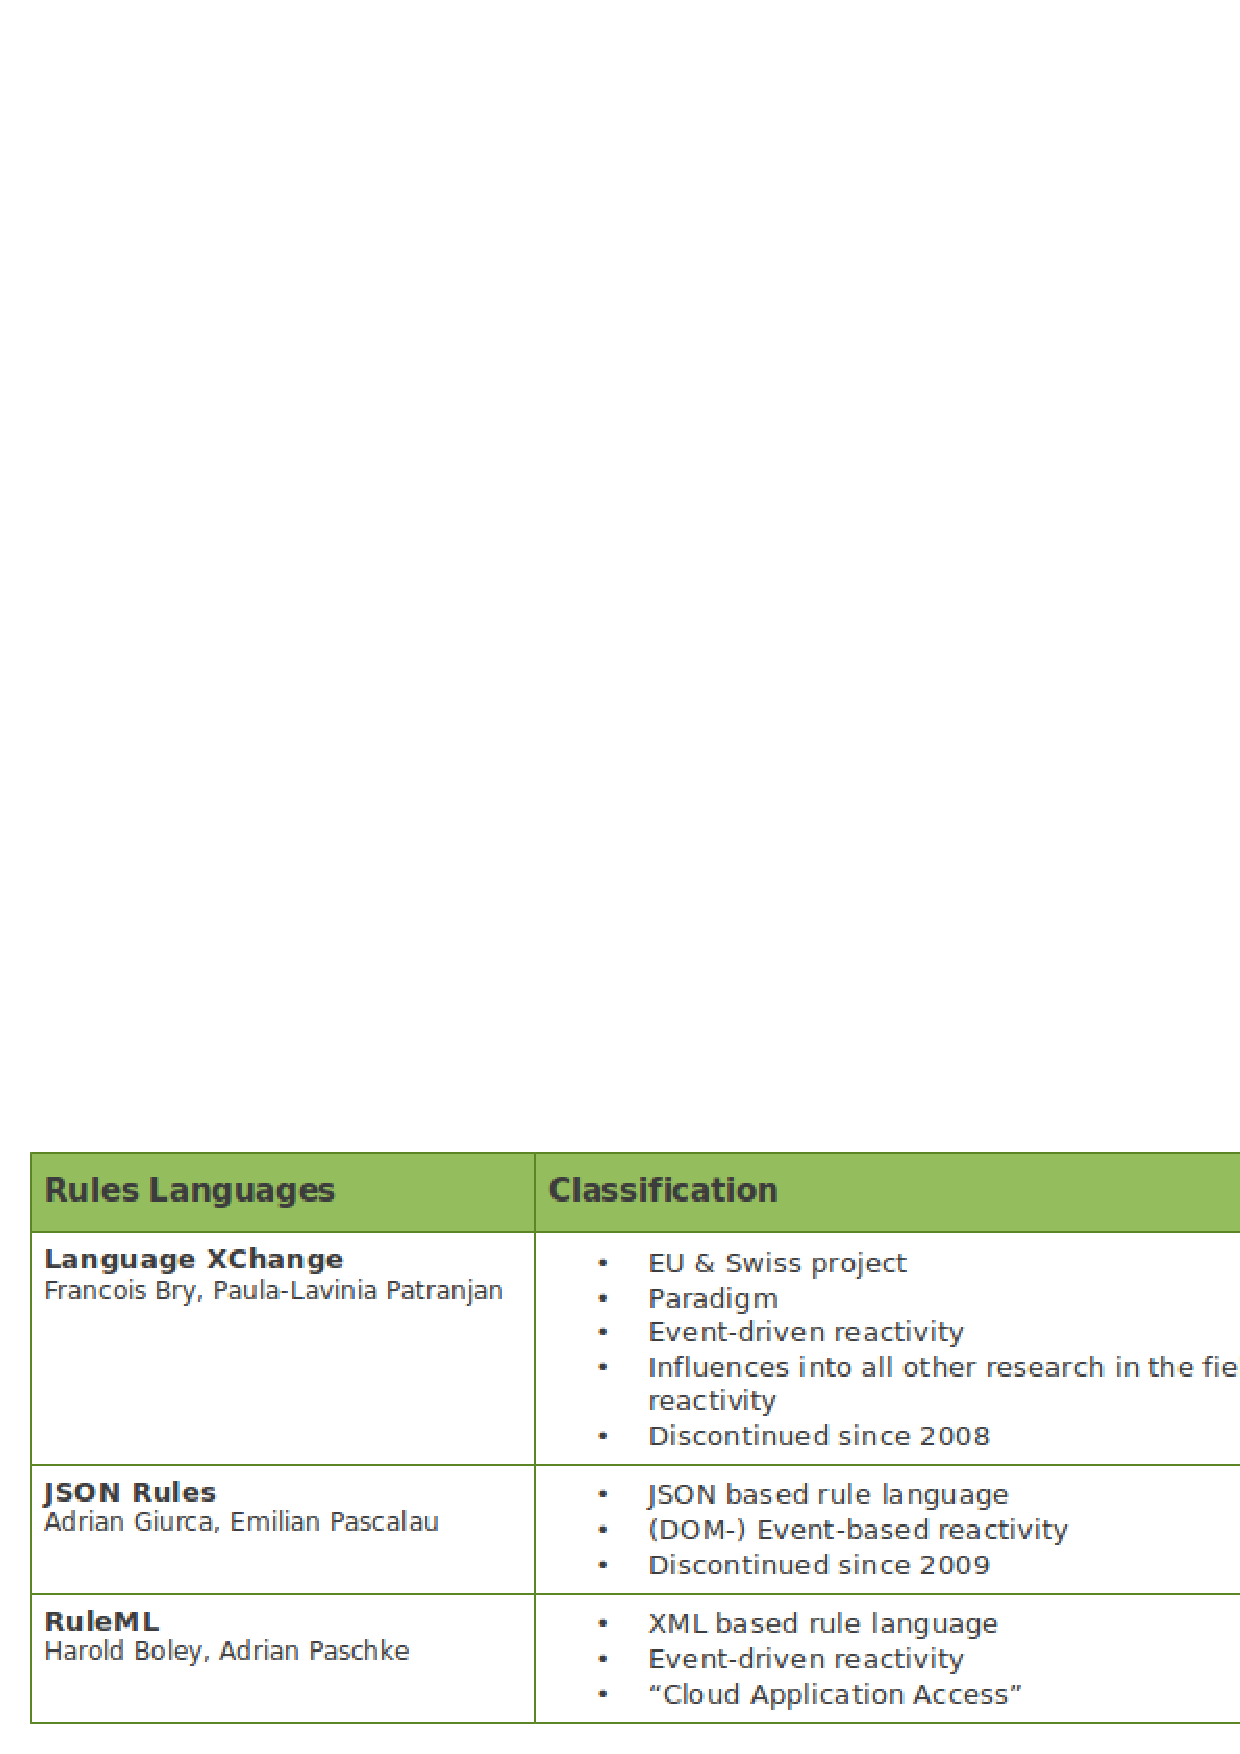
\includegraphics[scale=0.6]{img_rw_1_large}}%

\caption{Examined Rules Languages }
%\end{center}
\end{figure*}


\subsection{Rules Engines}
\subsubsection{(OO) jDrew}
Java Deductive Reasoning Engine for the Web (\emph{jDrew}~\cite{wwwjdrew}) is a reasoning engine written in Java for definite clause reasoning. jDrew can be embedded into larger systems through its APIs.
Object-Oriented jDrew (\emph{OO jDrew}~\cite{2005-Ball_etal-OOjDrew.pdf,wwwoojdrew}) is a Java based rule engine, it serves as a reference implementation of \emph{RuleML}. This project seems not to be very actively developed.

\subsubsection{Prova}
\emph{Prova}~\cite{wwwprova} is an expressive rule language and engine, both written in Java, with a main orientation to ECA rules. It uses backward-reasoning logic to formalize decisions in terms of derivation. Forward-directed messaging of reaction rules supports distributed event and action processing. It allows dynamic access to external data sources and is used by the authors of \cite{2013_Zhao-Paschke_EDSWE.pdf,2007-Paschke_etal-RuleResponder.pdf} for the \emph{RuleResponder's} proof of concept for transformations between different rule languages over \emph{RuleML}. \emph{Prova} seems to be discontinued since early 2013. 

\subsubsection{Kinetic}
The Kinetic Rules Engine (KRE) is a platform presented in \cite{bookTheLiveWeb}. It is realized in Perl and uses its very own rule language, the Kinetic Rules Language (KRL). It is laid out to support CEP as well as a tight coupling with the user's browser through plugins or libraries loaded via the webpage. It allows the access to remote resources and the processing of such data before passing it along to internal storage or again external resources, such as cloud applications. A live system~\cite{wwwkynetx} is available for testing and if desired also for productive use. Creating an own instance is quite a challenge due to it's numerous libraries. KRL needs quite some efforts to get used to and can't be entrusted to inexperienced users, thus a layer on top of this system would have to be implemented for our purposes.

\subsubsection{Drools Fusion}
\emph{Drools Fusion}~\cite{wwwdrools} is part of the jBoss open source community and allows the application of CEP and development in an eclipse-based IDE. Recently \emph{Drools 5} introduced the Business Logic integration Platform which provides a platform for Rules, Workflow and Event Processing. \emph{Drools Fusion} has its own rule language, \emph{Drools Rule Language (DRL)} This system has quite a heavy foot print, but active development is promising for a certain future stability.

\subsubsection{Rule Responder}
\emph{Rule Responder}~\cite{2007-Paschke_etal-RuleResponder.pdf} is a project to extend the Semantic Web towards a Pragmatic Web infrastructure for collaborative human-computer networks, which they call an architecture of a Pragmatic Agent Web (PAW). It supports the formation of virtual groupings and allows semi-automated agents with their individual contexts, decisions and actions. The authors postulate agents empowered with automatic rule-driven data transformation, decision derivation from existing knowledge and reaction according to changed situations or occurred events. The work done in this project concentrates on a layer on top of a rule engine and language, and thus allows for a combination of arbitrary rule-based systems via their framework. This is achieved through the usage of general message oriented communication interfaces and a platform-independent rule interchange format (\emph{RuleML}).

The authors of Rule Responder built their reference system\cite{wwwruleresponder} on top of the Mule~\cite{wwwmuleesb} open-source Enterprise Service Bus (ESB) which acts as a communication middleware. The decision to use Mule was made because it goes beyond the typical definition of an ESB by providing a distributable object broker to manage all sorts of service components. Each agent runs its own arbitrary rule engine. For demonstration purposes \emph{Prova} and \emph{OO jDrew} were used to demonstrate the rule interchange between different rule engines.

As research continued in terms of reaction rules and \textit{Rule Responder}, the authors of \cite{2013_Zhao-Paschke_EDSWE.pdf} showed the adoption of event paradigms to support scientific workflow execution. In their work they point out the limitations of ECA frameworks when adapted to their use case. For highly distributed and loosely coupled scientific workflows, complicated conditional procedures and rules, which can also have local scopes, are required. This shows us their work is going towards large distributed systems with a highly developed rule language that subsumes research from several fields.

\begin{figure*}[htb]
%\begin{center}
\centering
%,angle=-90
  \makebox[\textwidth][c]{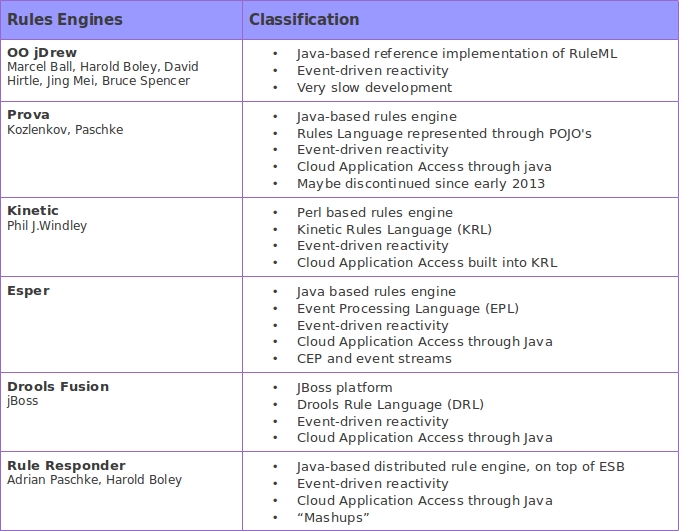
\includegraphics[scale=0.6]{img_rw_2_large}}%

\caption{Examined Rules Engines}
%\end{center}
\end{figure*}

\subsection{Mashups}
In \cite{2011-Pascalau-MBC.pdf}, one of the founders of \emph{JSON Rules} proposes to look at mashups as user-behaviour in a certain context. A mashup, to achieve a user-defined goal, is modelled via Unified Modeling Language (UML) as a map containing contexts and behaviour descriptions. Concepts are defined as unit of knowledge created by unique combination of characteristics. Contexts are defined as a set of concepts. A mashup is then defined as  set of contexts behaviour, where behaviour consists of rules and processes. The conceptual work done in this paper is interesting but the promoted example isn't accessible.

It is also important to understand what users expect from service mashups, in order to provide a useful platform to them. In \cite{2010-Namoun_etal-EURCW.pdf} research is done in identifying user perceptions of services, their composition, user working ways and expectations towards a composition tool. They come up with a set of recommendations to aid the development of mashup environments. A survey~\cite{2009-Fischer_etal-OCAMG.pdf} that went into a similar direction categorizes the different frameworks for user driven mashup development as based on:
 \begin{itemize}
%\itemsep-1.5em
  \item Programming Paradigm
  \item Scripting Languages
  \item Spreadsheets
  \item Wiring Paradigm
  \item Programming by Demonstration
  \item Automatic Creation of Mashups
\end{itemize}
But even though large efforts are made in all these research fields, inexperienced users are still not able to build mashups without knowledge about numerous aspects of the framework or programming.

\subsubsection{useKit}
The idea of \emph{useKit}~\cite{2010-Rizzotti_Burkhart-useKit.pdf} missions shows us the potential of user-manageable cloud application mashups. While their approach is not event-based, it can be regarded as a base for the web's evolution towards user-programmable reactive cloud application mashups.

\subsubsection{DashMash}
The DashMash~\cite{2011-Cappiello_etal-DashMash.pdf} platform is an approach to give end-users the graphical tools in a browser to mash up web applications in a dashboard. A resource of (for stability reasons) trimmed services (such as GoogleMaps or TripAdvisor), filters, viewers and generic components is accessible to the users. DashMash uses an event-driven model of the presentation level, similar to a JSON Rules approach in \cite{2009-Pascalau_Giurca-RBACEM.pdf}. There are events sent by the client to the server, but they are only used to update all viewers with the actual data the user is looking at.

\begin{figure*}[htb]
%\begin{center}
\centering
%,angle=-90
  \makebox[\textwidth][c]{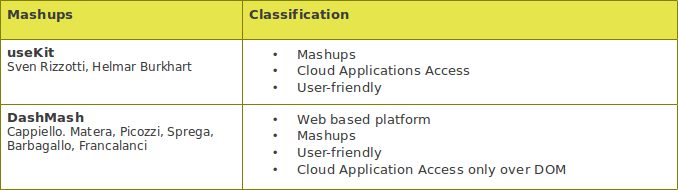
\includegraphics[scale=0.6]{img_rw_3_large}}%

\caption{Examined Mashup Approaches}
%\end{center}
\end{figure*}

\section{Use Case Study}
In order to verify some of the identified related work, use cases around the successor of useKit~\cite{2010-Rizzotti_Burkhart-useKit.pdf} (ProBinder~\cite{wwwprobinder}) have been derived and investigated. 
Three use cases have been identified to verify the feasibility of certain existing infrastructures.

\subsection{Binder Watcher}
Binder Watcher is about binders being watched and actions that are taken after certain changes to a binder. Users of ProBinder, which are involved in many different companies and project binders, tend to be confronted with a large amount of information. It is a tedious task to get the user's context back into a clean state, where the ProBinder system is ready to reflect new recent changes in an optimal way to the user. By allowing the users to identify resources (binder tabs in this case, but it could also be complete binders, persons, companies, \dots) of interest, the user task can be automated to a certain extent. As soon as changes are made to the resources of interest, they are marked as read and summarized. These summaries are then provided to the user, which allows him to identify the most important changes.

The Binder Watcher use case was implemented in KRL (see \ref{app:uc_bw_krl}) and provided the important insight that the realization of such a use case in an ECA is a time-consuming challenge. 

\subsection{Activating Legacy Resources}
To bring reactivity to the static web, we have to enhance legacy resources, which are not event-ready. Changes in such resources have to be detected via e.g. web spiders or crawlers and transformed into events that can be processed by the rules engine. Such an auxiliary cloud application would turn the static web into a reactive system and free a future architecture from incorporating the pulling of events, thus allowing it to concentrate on its main business, i.e. event handling.

\subsubsection{From the Web to the Cloud}
To make the static web active, an \emph{activator} monitors a predefined remote resource, e.g. a public ProBinder tab, accessed via the normal webpage, not the API. Changes to the tab are detected and pushed into the event-based system as events. In our case we built a reference system on top of \emph{node.js}. These events then have to be processed according to rules and finally actions are invoked, which could also be events again. For our study the action taken was again \emph{ProBinder} which was used to create an entry in another binder, this time via the API. This use case was mainly used to proof the accessibility of ProBinder via a remote system and the activation of the static web.

\subsubsection{From the Cloud to the Web}
Since cloud applications already provide quite a lot of notifications, they offer themselves as event producers. But most of todays notifications are received by pulling. Only few offer the possibility to register webhooks where they would push events to. The number of cloud applications that offer webhooks will most likely increase in the future and continue to make the web more reactive. But for now after dealing with the static web in the use case above, we need to deal with a semi-reactive web as well. These pull requests to such resources could again be taken care of by introducing an \emph{activator}, which polls periodically for updates and pushes them into the even-based system. 
Now the system is able to check these events for conditions and invokes actions according to existing rules.

If we have the static web as an action destination, the question is how a static resource is going to react to such an action invocation. There are basically three possibilities to that, first we could implement an interface to the provider of the static resource in order to really change the resource, visible for every body in the web.
Secondly, we simulate reactivity through our system. Actions taken on behalf of such a resource are stored in an internal state representation of the resource and if certain rules are met, the simulator could produce again events. Each user that is connected to our system, would then be able to experience this reactivity of static resources, and eventually also if other users interacted with the system.
The third possibility is, rules could also run in a lightweighted architecture on the client browser, which influences the DOM tree to existing rules. Like this it would be easier to maintain a private view for users, but state changes could only be maintained during the browser sessions. Storing these state changes on the server side of the event-based system could overcome that shortfall and a combined solution seems to be a good proof of concept strategy. 

\subsubsection{Node.js}
In order to implement some proof of concept examples, \emph{node.js} was used as a basis to implement a custom module.
\emph{node.js} is a powerful tool to build cloud applications. Because of its modularity and the package manager, slim instances can be run. Its main purpose is to be used as a webserver. By incorporating JavaScript's asynchronous design of callback functions into their architecture, locking situations are basically omitted. Thus it is a highly-scalable, asynchronous, event-driven architecture which found broad acceptance in the open-source comunity as well as for enterprises.

The package manager \emph{npm} can be used to maintain dependencies of a custom \emph{node.js} module to other modules. This helpful feature ensures that everybody working with the user-defined module uses the same external modules and the respective versions. Also project repositories do not need to store the dependent libraries through this mechanism, thus saving space and traffic. 
A name and a version are mandatory for a \emph{node.js} module. Knowing the name, e.g. \PY{n}{diff}, one can look up the latest version in the \emph{npm} repository by issuing following command:

\begin{Verbatim}[commandchars=\\\{\}]
\PY{err}{\PYZdl{}} \PY{n}{npm} \PY{n}{show} \PY{n}{diff} \PY{n}{version}
\PY{n}{npm} \PY{n}{http} \PY{n}{GET} \PY{n}{https}\PY{p}{:}\PY{o}{/}\PY{o}{/}\PY{n}{registry}\PY{o}{.}\PY{n}{npmjs}\PY{o}{.}\PY{n}{org}\PY{o}{/}\PY{n}{diff}
\PY{n}{npm} \PY{n}{http} \PY{l+m+mi}{200} \PY{n}{https}\PY{p}{:}\PY{o}{/}\PY{o}{/}\PY{n}{registry}\PY{o}{.}\PY{n}{npmjs}\PY{o}{.}\PY{n}{org}\PY{o}{/}\PY{n}{diff}
\PY{l+m+mf}{1.0}\PY{o}{.}\PY{l+m+mi}{5}
\end{Verbatim}


Now this dependency, together with the version one would like to use, can be inserted into the own project description file as shown below.
For our small use case proof of concept project we only had to define the project description file called \PY{n}{package.json} in the root folder of the project:

\begin{Verbatim}[commandchars=\\\{\}]
\PY{p}{\PYZob{}}
	\PY{l+s+s2}{\PYZdq{}name\PYZdq{}}\PY{o}{:} \PY{l+s+s2}{\PYZdq{}msc\PYZhy{}apps\PYZdq{}}\PY{p}{,}
	\PY{l+s+s2}{\PYZdq{}description\PYZdq{}}\PY{o}{:} \PY{l+s+s2}{\PYZdq{}Proof of concept apps\PYZdq{}}\PY{p}{,}
	\PY{l+s+s2}{\PYZdq{}version\PYZdq{}}\PY{o}{:} \PY{l+s+s2}{\PYZdq{}0.0.1\PYZdq{}}\PY{p}{,}
	\PY{l+s+s2}{\PYZdq{}private\PYZdq{}}\PY{o}{:} \PY{k+kc}{true}\PY{p}{,}
	\PY{l+s+s2}{\PYZdq{}dependencies\PYZdq{}}\PY{o}{:} \PY{p}{\PYZob{}}
	\PY{l+s+s2}{\PYZdq{}request\PYZdq{}}\PY{o}{:} \PY{l+s+s2}{\PYZdq{}2.22.0\PYZdq{}}\PY{p}{,}
	\PY{l+s+s2}{\PYZdq{}express\PYZdq{}}\PY{o}{:} \PY{l+s+s2}{\PYZdq{}3.3.4\PYZdq{}}\PY{p}{,}
	\PY{l+s+s2}{\PYZdq{}diff\PYZdq{}}\PY{o}{:} \PY{l+s+s2}{\PYZdq{}1.0.5\PYZdq{}}
	\PY{p}{\PYZcb{}}
\PY{p}{\PYZcb{}}
\end{Verbatim}

Everybody who downloads this project needs to download the dependencies before using the module. This is done by running following command in the root directory of the project:
\begin{Verbatim}[commandchars=\\\{\}]
\PY{err}{\PYZdl{}} \PY{n}{npm} \PY{n}{install}
\end{Verbatim}
If any dependencies change in the future the same command can be run again to update the local project.
A simple Hello World example of \emph{node.js} looks like this:
\begin{Verbatim}[commandchars=\\\{\}]
\PY{k+kd}{var} \PY{n+nx}{http} \PY{o}{=} \PY{n+nx}{require}\PY{p}{(}\PY{l+s+s1}{\PYZsq{}http\PYZsq{}}\PY{p}{)}\PY{p}{;}
\PY{k+kd}{var} \PY{n+nx}{server} \PY{o}{=} \PY{n+nx}{http}\PY{p}{.}\PY{n+nx}{createServer}\PY{p}{(}\PY{k+kd}{function} \PY{p}{(}\PY{n+nx}{request}\PY{p}{,} \PY{n+nx}{response}\PY{p}{)} \PY{p}{\PYZob{}}
  \PY{n+nx}{response}\PY{p}{.}\PY{n+nx}{writeHead}\PY{p}{(}\PY{l+m+mi}{200}\PY{p}{,} \PY{p}{\PYZob{}}\PY{l+s+s2}{\PYZdq{}Content\PYZhy{}Type\PYZdq{}}\PY{o}{:} \PY{l+s+s2}{\PYZdq{}text/plain\PYZdq{}}\PY{p}{\PYZcb{}}\PY{p}{)}\PY{p}{;}
  \PY{n+nx}{response}\PY{p}{.}\PY{n+nx}{end}\PY{p}{(}\PY{l+s+s2}{\PYZdq{}Hello World\PYZbs{}n\PYZdq{}}\PY{p}{)}\PY{p}{;}
\PY{p}{\PYZcb{}}\PY{p}{)}\PY{p}{;}
\PY{n+nx}{server}\PY{p}{.}\PY{n+nx}{listen}\PY{p}{(}\PY{l+m+mi}{8000}\PY{p}{)}\PY{p}{;}
\end{Verbatim}

After executing this by typing (if the above code was stored in a file called \PY{n}{index.js})
\begin{Verbatim}[commandchars=\\\{\}]
\PY{err}{\PYZdl{}} \PY{n}{node} \PY{n}{index.js}
\end{Verbatim}
the webserver is accessible on port 8000 (by typing \PY{n}{localhost:8000} in the browser bar), and responds with ''Hello World''.
Examples of the use case implementations in \emph{node.js} can be found in the appendix.

\section{Conclusion}
In \cite{2009-Pascalau_Giurca-LWAECARE.pdf}, the founders of \emph{JSON Rules}~\cite{2008-Giurca_Pascalau-JSON_Rules.pdf} describe a lightweight architecture that allows to react and proact on behalf of events in the ontology of web browsers. \emph{JSON Rules} is promising for our work because of its lightweight architecture and specialization on production and ECA rules. But the existing working memory architecture needs to be generalized to allow a different environment, other than just the DOM tree. The existing architecture could be used to allow the user to create local rules that do not access remote systems and thus runs into authentication issues.

Other approaches are server side rule engines either written in Perl or Java, where powerful tools are provided to process events and invoke manifold actions. But these approaches all lack an abstraction layer to introduce the programmability of the reactive web to a large audience of inexperienced users. Also, current approaches concentrate on data flows instead of event flows, thus not incorporating reactivity to the web.

With \emph{RuleML} a powerful, interchangeable expression language for event-based systems is present. It paves the way for distributed rule engines, such as one running in the browser and another on a server for cloud application access. But a rule engine that incorporates the requirements of a lightweighted architecture and user-readiness is missing. Under related work, \cite{2010-Namoun_etal-EURCW.pdf} pointed out the difficulties of inexperienced users to tackle the execution flow. This issue arose from their approach of displaying all services as very similar UI's. By introducing an event-based system, event producers would be clearly different from action consumers. This would address this issue in an user-intuitive way.

Large systems such as \emph{RuleResponder} weave stubs or proxies of existing service into a message oriented middleware (MoM). We envision the web itself is used as the middleware. Through this a lightweighted and performant event-based architecture can be realized, which allows the orchestration of existing web and cloud applications.

\section{Future Work}
Developing an event-driven architecture which regards cloud applications as event-based first-class citizens and allows for an intuitive user-driven mashup development is a research field that has, to the best of our knowledge, not been addressed yet. Looking at cloud-based applications as event producers and action consumers gives new ways to bring reactivity into the existing web. Such representations require a rule-based system that allows their interweaving. Not solely the interaction between cloud applications should be addressed, but also with the browser itself, since it is a tool which is predominantly used to access the web. This would empower the user to predefine influences and interactions on existing cloud applications before they are accessed, providing novel powerful ways to govern the web.

Since the vision of on- and offline rules can't be covered with a single server application, the utilization of a fast, flexible and widely used technology such as JavaScript to tackle this challenge seems to be favorable future work. JavaScript was mainly invented for browsers and is spread all over the web by now. Additionally, applications such as \emph{node.js}~\cite{wwwnodejs}, bring JavaScript to the server-side and tear down the communication efforts between cloud applications through JSON messages which are directly understood by modern browsers and cloud applications.
Preferably a lightweighted rules engine would be used to run the user-generated mashups. The KRE suits the demand for a certain coupling between the users browser and the remote rules engine to provide a powerful system. On the other hand the rules engine is not (yet) well documented, not lightweighted and forged in Perl, a programming language that wasn't encountered during the research for related work on rule based systems.

Sharing and thus exchanging of rules gives new ways for collaboration and the possibility for expert users to aid less experienced ones, giving them the chance to catch up with the future platform. 
In terms of usability an easy to understand way to create rules would have a large benefit. We envision a graphical toolkit that empowers users to build their own complex event-based cloud application mashups, powerful RIAs.
A first approach could be to write rules in a certain language, e.g. \emph{RuleML} or \emph{JSON Rules}, then simplify the vocabulary until meaningful graphical representations are possible.

It is striking but not surprising, that all related work we looked at, only used public cloud applications, thus omitting the challenge of authorization and the safety of the user's private context.
If users are provided the tools to access public cloud APIs and create mashups with them, they are going to benefit from this. But mostly users these days are traveling in the web within their private, secured context. Thus the access to such resources are providing even more power- and meaningful tools to the user. The future reactive web requires cloud applications that allow the registration of webhooks in order for the rules engine to receive events from resources other than the own system, thus using the internet as middleware for communication of push events.

\bibliography{liveweb}
\bibliographystyle{related-work}

\newpage
\appendix
\lstset { basicstyle=\tiny }
\renewcommand\thesection{Appendix \Alph{section}}

\section{Binder Watcher KRL code} \label{app:uc_bw_krl}
\begin{Verbatim}[fontsize=\scriptsize,commandchars=\\\{\}]
\PY{n}{ruleset} \PY{n}{a2236x4} \PY{p}{\PYZob{}}
  \PY{n}{meta} \PY{p}{\PYZob{}}
    \PY{n}{name} \PY{l+s}{\PYZdq{}}\PY{l+s}{ProBinder Flag Notification Handler}\PY{l+s}{\PYZdq{}}
    \PY{n}{description} \PY{l+s}{\PYZdq{}}\PY{l+s}{This is a first example on how to react on ProBinder Events}\PY{l+s}{\PYZdq{}}
    \PY{n}{author} \PY{l+s}{\PYZdq{}}\PY{l+s}{dominic.bosch}\PY{l+s}{\PYZdq{}}
    \PY{o}{/}\PY{o}{/}\PY{n}{ProBinder} \PY{n}{IDs}\PY{p}{:}
    \PY{o}{/}\PY{o}{/} \PY{n}{userID}\PY{p}{:} \PY{l+m+mi}{10595}
    \PY{o}{/}\PY{o}{/} \PY{n}{companyID}\PY{p}{:} \PY{l+m+mi}{643}
    \PY{o}{/}\PY{o}{/} \PY{n}{contextID}\PY{p}{:} \PY{l+m+mi}{16694}
    \PY{o}{/}\PY{o}{/} \PY{n}{followerID}\PY{p}{:} \PY{l+m+mi}{12613}
    
    \PY{n}{logging} \PY{n}{on}
  \PY{p}{\PYZcb{}}
  
  \PY{n}{dispatch} \PY{p}{\PYZob{}}\PY{p}{\PYZcb{}}
  
  \PY{k}{global} \PY{p}{\PYZob{}}\PY{p}{\PYZcb{}}
  
  \PY{o}{/}\PY{o}{/} \PY{n}{Reset} \PY{n}{all} \PY{n}{entitiy} \PY{n}{variables}
  \PY{n}{rule} \PY{n}{resetAll} \PY{p}{\PYZob{}}
    \PY{n}{select} \PY{n}{when} \PY{n}{probinder} \PY{n}{resetall}
      \PY{n}{send\PYZus{}directive}\PY{p}{(}\PY{l+s}{\PYZdq{}}\PY{l+s}{Full Reset}\PY{l+s}{\PYZdq{}}\PY{p}{)}\PY{p}{;}
      \PY{n}{fired} \PY{p}{\PYZob{}}
        \PY{n}{clear} \PY{n}{ent}\PY{p}{:}\PY{n}{userID}\PY{p}{;}
        \PY{n}{clear} \PY{n}{ent}\PY{p}{:}\PY{n}{companyID}\PY{p}{;}
        \PY{n}{clear} \PY{n}{ent}\PY{p}{:}\PY{n}{contextID}\PY{p}{;}
        \PY{n}{clear} \PY{n}{ent}\PY{p}{:}\PY{n}{credentials}\PY{p}{;}
        \PY{n}{clear} \PY{n}{ent}\PY{p}{:}\PY{n}{followers}\PY{p}{;}
        \PY{n}{clear} \PY{n}{ent}\PY{p}{:}\PY{n}{newContents}\PY{p}{;}
        \PY{n}{clear} \PY{n}{ent}\PY{p}{:}\PY{n}{summary}\PY{p}{;}
        \PY{n}{clear} \PY{n}{ent}\PY{p}{:}\PY{n}{temp}\PY{p}{;}
      \PY{p}{\PYZcb{}}
  \PY{p}{\PYZcb{}}
  
  \PY{o}{/}\PY{o}{/} \PY{n}{reset} \PY{n}{the} \PY{n}{unread} \PY{n}{content} \PY{n}{data} \PY{n}{structures}
  \PY{n}{rule} \PY{n}{reset} \PY{p}{\PYZob{}}
    \PY{n}{select} \PY{n}{when} \PY{n}{probinder} \PY{n}{reset}
      \PY{n}{send\PYZus{}directive}\PY{p}{(}\PY{l+s}{\PYZdq{}}\PY{l+s}{Reset, user credentials and followers still kept}\PY{l+s}{\PYZdq{}}\PY{p}{)}\PY{p}{;}
      \PY{n}{fired} \PY{p}{\PYZob{}}
        \PY{n}{clear} \PY{n}{ent}\PY{p}{:}\PY{n}{newContents}\PY{p}{;}
        \PY{n}{clear} \PY{n}{ent}\PY{p}{:}\PY{n}{summary}\PY{p}{;}
        \PY{n}{clear} \PY{n}{ent}\PY{p}{:}\PY{n}{temp}\PY{p}{;}
      \PY{p}{\PYZcb{}}
  \PY{p}{\PYZcb{}}
  
  \PY{o}{/}\PY{o}{/} \PY{n}{The} \PY{n}{user} \PY{n}{registers} \PY{n}{himself} \PY{n}{with} \PY{n}{email} \PY{n}{and} \PY{n}{password} \PY{n}{for} \PY{n}{the} \PY{n}{ProBinder} \PY{n}{API}\PY{o}{.}\PY{o}{.}\PY{o}{.}
  \PY{n}{rule} \PY{n}{register\PYZus{}user} \PY{p}{\PYZob{}}
    \PY{n}{select} \PY{n}{when} \PY{n}{probinder} \PY{n}{register}
      \PY{k}{if} \PY{p}{(}\PY{n}{event}\PY{p}{:}\PY{n}{attr}\PY{p}{(}\PY{l+s}{\PYZsq{}}\PY{l+s}{userID}\PY{l+s}{\PYZsq{}}\PY{p}{)}\PY{o}{.}\PY{k}{as}\PY{p}{(}\PY{l+s}{\PYZdq{}}\PY{l+s}{str}\PY{l+s}{\PYZdq{}}\PY{p}{)} \PY{n}{neq} \PY{l+s}{\PYZsq{}}\PY{l+s}{null}\PY{l+s}{\PYZsq{}}
          \PY{o}{\PYZam{}}\PY{o}{\PYZam{}} \PY{n}{event}\PY{p}{:}\PY{n}{attr}\PY{p}{(}\PY{l+s}{\PYZsq{}}\PY{l+s}{companyID}\PY{l+s}{\PYZsq{}}\PY{p}{)}\PY{o}{.}\PY{k}{as}\PY{p}{(}\PY{l+s}{\PYZdq{}}\PY{l+s}{str}\PY{l+s}{\PYZdq{}}\PY{p}{)} \PY{n}{neq} \PY{l+s}{\PYZsq{}}\PY{l+s}{null}\PY{l+s}{\PYZsq{}}
          \PY{o}{\PYZam{}}\PY{o}{\PYZam{}} \PY{n}{event}\PY{p}{:}\PY{n}{attr}\PY{p}{(}\PY{l+s}{\PYZsq{}}\PY{l+s}{contextID}\PY{l+s}{\PYZsq{}}\PY{p}{)}\PY{o}{.}\PY{k}{as}\PY{p}{(}\PY{l+s}{\PYZdq{}}\PY{l+s}{str}\PY{l+s}{\PYZdq{}}\PY{p}{)} \PY{n}{neq} \PY{l+s}{\PYZsq{}}\PY{l+s}{null}\PY{l+s}{\PYZsq{}}
          \PY{o}{\PYZam{}}\PY{o}{\PYZam{}} \PY{n}{event}\PY{p}{:}\PY{n}{attr}\PY{p}{(}\PY{l+s}{\PYZsq{}}\PY{l+s}{email}\PY{l+s}{\PYZsq{}}\PY{p}{)}\PY{o}{.}\PY{k}{as}\PY{p}{(}\PY{l+s}{\PYZdq{}}\PY{l+s}{str}\PY{l+s}{\PYZdq{}}\PY{p}{)} \PY{n}{neq} \PY{l+s}{\PYZsq{}}\PY{l+s}{null}\PY{l+s}{\PYZsq{}}
          \PY{o}{\PYZam{}}\PY{o}{\PYZam{}} \PY{n}{event}\PY{p}{:}\PY{n}{attr}\PY{p}{(}\PY{l+s}{\PYZsq{}}\PY{l+s}{password}\PY{l+s}{\PYZsq{}}\PY{p}{)}\PY{o}{.}\PY{k}{as}\PY{p}{(}\PY{l+s}{\PYZdq{}}\PY{l+s}{str}\PY{l+s}{\PYZdq{}}\PY{p}{)} \PY{n}{neq} \PY{l+s}{\PYZsq{}}\PY{l+s}{null}\PY{l+s}{\PYZsq{}}\PY{p}{)} \PY{n}{then} \PY{p}{\PYZob{}}
        \PY{n}{send\PYZus{}directive}\PY{p}{(}\PY{l+s}{\PYZdq{}}\PY{l+s}{user registered}\PY{l+s}{\PYZdq{}}\PY{p}{)}\PY{p}{;}
      \PY{p}{\PYZcb{}}
      \PY{n}{fired} \PY{p}{\PYZob{}}
        \PY{n+nb}{set} \PY{n}{ent}\PY{p}{:}\PY{n}{userID} \PY{n}{event}\PY{p}{:}\PY{n}{attr}\PY{p}{(}\PY{l+s}{\PYZsq{}}\PY{l+s}{userID}\PY{l+s}{\PYZsq{}}\PY{p}{)}\PY{p}{;}
        \PY{n+nb}{set} \PY{n}{ent}\PY{p}{:}\PY{n}{companyID} \PY{n}{event}\PY{p}{:}\PY{n}{attr}\PY{p}{(}\PY{l+s}{\PYZsq{}}\PY{l+s}{companyID}\PY{l+s}{\PYZsq{}}\PY{p}{)}\PY{p}{;}
        \PY{n+nb}{set} \PY{n}{ent}\PY{p}{:}\PY{n}{contextID} \PY{n}{event}\PY{p}{:}\PY{n}{attr}\PY{p}{(}\PY{l+s}{\PYZsq{}}\PY{l+s}{contextID}\PY{l+s}{\PYZsq{}}\PY{p}{)}\PY{p}{;}
        \PY{n+nb}{set} \PY{n}{ent}\PY{p}{:}\PY{n}{credentials} \PY{n}{uri}\PY{p}{:}\PY{n}{escape}\PY{p}{(}\PY{n}{event}\PY{p}{:}\PY{n}{attr}\PY{p}{(}\PY{l+s}{\PYZsq{}}\PY{l+s}{email}\PY{l+s}{\PYZsq{}}\PY{p}{)}\PY{p}{)} \PY{o}{+} \PY{l+s}{\PYZdq{}}\PY{l+s}{:}\PY{l+s}{\PYZdq{}} \PY{o}{+} \PY{n}{uri}\PY{p}{:}\PY{n}{escape}\PY{p}{(}\PY{n}{event}\PY{p}{:}\PY{n}{attr}\PY{p}{(}\PY{l+s}{\PYZsq{}}\PY{l+s}{password}\PY{l+s}{\PYZsq{}}\PY{p}{)}\PY{p}{)}\PY{p}{;}
      \PY{p}{\PYZcb{}}
  \PY{p}{\PYZcb{}}
  
  \PY{o}{/}\PY{o}{/} \PY{n}{The} \PY{n}{user} \PY{n}{sent} \PY{n}{an} \PY{n}{event} \PY{n}{that} \PY{n}{tells} \PY{n}{us} \PY{n}{he} \PY{n}{wants} \PY{n}{to} \PY{n}{follow} \PY{n}{somebody}
  \PY{n}{rule} \PY{n}{new\PYZus{}user\PYZus{}to\PYZus{}follow} \PY{p}{\PYZob{}}
    \PY{n}{select} \PY{n}{when} \PY{n}{probinder} \PY{n}{newfollower}
      \PY{n}{pre}\PY{p}{\PYZob{}}
        \PY{n}{listFollowers} \PY{o}{=} \PY{n}{ent}\PY{p}{:}\PY{n}{followers} \PY{o}{|}\PY{o}{|} \PY{p}{\PYZob{}}\PY{p}{\PYZcb{}}\PY{p}{;}
        \PY{n}{newfollower} \PY{o}{=} \PY{n}{event}\PY{p}{:}\PY{n}{attr}\PY{p}{(}\PY{l+s}{\PYZsq{}}\PY{l+s}{followerID}\PY{l+s}{\PYZsq{}}\PY{p}{)}\PY{o}{.}\PY{k}{as}\PY{p}{(}\PY{l+s}{\PYZdq{}}\PY{l+s}{str}\PY{l+s}{\PYZdq{}}\PY{p}{)}\PY{p}{;}
        \PY{n}{listFollowers} \PY{o}{=} \PY{n}{listFollowers}\PY{o}{.}\PY{n}{put}\PY{p}{(}\PY{p}{[}\PY{n}{newfollower}\PY{p}{]}\PY{p}{,} \PY{l+s}{\PYZdq{}}\PY{l+s}{true}\PY{l+s}{\PYZdq{}}\PY{p}{)}\PY{p}{;}
      \PY{p}{\PYZcb{}}
      \PY{k}{if} \PY{p}{(}\PY{n}{event}\PY{p}{:}\PY{n}{attr}\PY{p}{(}\PY{l+s}{\PYZsq{}}\PY{l+s}{userID}\PY{l+s}{\PYZsq{}}\PY{p}{)} \PY{o}{==} \PY{n}{ent}\PY{p}{:}\PY{n}{userID}
          \PY{o}{\PYZam{}}\PY{o}{\PYZam{}} \PY{n}{newfollower} \PY{n}{neq} \PY{l+s}{\PYZdq{}}\PY{l+s}{null}\PY{l+s}{\PYZdq{}}\PY{p}{)} \PY{n}{then} \PY{p}{\PYZob{}}
            \PY{n}{send\PYZus{}directive}\PY{p}{(}\PY{l+s}{\PYZdq{}}\PY{l+s}{New ProBinder User added to followers}\PY{l+s}{\PYZdq{}}\PY{p}{)}\PY{p}{;}
      \PY{p}{\PYZcb{}}
      \PY{n}{fired}\PY{p}{\PYZob{}}
        \PY{n+nb}{set} \PY{n}{ent}\PY{p}{:}\PY{n}{followers} \PY{n}{listFollowers}
      \PY{p}{\PYZcb{}}
  \PY{p}{\PYZcb{}}
  
  \PY{o}{/}\PY{o}{/} \PY{n}{Let} \PY{n}{the} \PY{n}{KRE} \PY{n}{check} \PY{n}{ProBinder} \PY{n}{for} \PY{n}{new} \PY{n}{unread} \PY{n}{content} \PY{n}{and} \PY{n}{process} \PY{n}{it} \PY{n}{immediately}
  \PY{n}{rule} \PY{n}{check\PYZus{}for\PYZus{}unread\PYZus{}content} \PY{p}{\PYZob{}}
    \PY{n}{select} \PY{n}{when} \PY{n}{probinder} \PY{n}{check}
      \PY{n}{pre} \PY{p}{\PYZob{}}
        \PY{n}{r} \PY{o}{=} \PY{n}{http}\PY{p}{:}\PY{n}{get}\PY{p}{(}\PY{l+s}{\PYZdq{}}\PY{l+s}{https://}\PY{l+s}{\PYZdq{}} \PY{o}{+} \PY{n}{ent}\PY{p}{:}\PY{n}{credentials} \PY{o}{+} \PY{l+s}{\PYZdq{}}\PY{l+s}{@probinder.com/service/36/unreadcontent}\PY{l+s}{\PYZdq{}}\PY{p}{)}\PY{p}{;}
        \PY{n}{arr} \PY{o}{=} \PY{n}{r}\PY{p}{\PYZob{}}\PY{l+s}{\PYZdq{}}\PY{l+s}{content}\PY{l+s}{\PYZdq{}}\PY{p}{\PYZcb{}}\PY{o}{.}\PY{n}{decode}\PY{p}{(}\PY{p}{)}\PY{p}{;}
      \PY{p}{\PYZcb{}}
      \PY{n}{send\PYZus{}directive}\PY{p}{(}\PY{l+s}{\PYZdq{}}\PY{l+s}{Checked ProBinder for unread content, found: }\PY{l+s}{\PYZdq{}} \PY{o}{+} \PY{n}{arr}\PY{o}{.}\PY{n}{length}\PY{p}{(}\PY{p}{)}\PY{p}{)}\PY{p}{;}
      \PY{n}{fired} \PY{p}{\PYZob{}}
        \PY{n+nb}{set} \PY{n}{ent}\PY{p}{:}\PY{n}{newContents} \PY{n}{arr}\PY{p}{;}
        \PY{k}{raise} \PY{n}{explicit} \PY{n}{event} \PY{n}{processnewcontents}\PY{p}{;}
      \PY{p}{\PYZcb{}}
    
  \PY{p}{\PYZcb{}}
  
  \PY{o}{/}\PY{o}{/} \PY{n}{Work} \PY{p}{(}\PY{n}{new} \PY{n}{unread} \PY{n}{content}\PY{p}{)} \PY{n}{from} \PY{n}{ProBinder} \PY{n}{to} \PY{n}{process}
  \PY{n}{rule} \PY{n}{process\PYZus{}new\PYZus{}contents} \PY{p}{\PYZob{}}
    \PY{n}{select} \PY{n}{when} \PY{n}{explicit} \PY{n}{processnewcontents}
    \PY{o}{/}\PY{o}{/} \PY{n}{Process} \PY{n}{only} \PY{n}{the} \PY{n}{unread} \PY{n}{contents} \PY{n}{from} \PY{n}{people} \PY{n}{we} \PY{n}{are} \PY{n}{following}\PY{p}{,}
    \PY{o}{/}\PY{o}{/} \PY{n}{filter} \PY{n}{condition} \PY{n}{omits} \PY{n}{unnecessary} \PY{n}{rules} \PY{n}{invocation}
    \PY{n}{foreach} \PY{n}{ent}\PY{p}{:}\PY{n}{newContents}\PY{o}{.}\PY{n}{filter}\PY{p}{(}
      \PY{n}{function}\PY{p}{(}\PY{n}{d}\PY{p}{)} \PY{p}{\PYZob{}}\PY{n}{ent}\PY{p}{:}\PY{n}{followers}\PY{o}{.}\PY{n}{pick}\PY{p}{(}\PY{l+s}{\PYZdq{}}\PY{l+s}{\PYZdl{}.}\PY{l+s}{\PYZdq{}}\PY{o}{+}\PY{n}{d}\PY{o}{.}\PY{n}{pick}\PY{p}{(}\PY{l+s}{\PYZdq{}}\PY{l+s}{\PYZdl{}.userId}\PY{l+s}{\PYZdq{}}\PY{p}{)}\PY{p}{)} \PY{o}{!=} \PY{n}{null}\PY{p}{\PYZcb{}}
    \PY{p}{)} \PY{n}{setting}\PY{p}{(}\PY{n}{nc}\PY{p}{)}
      \PY{n}{pre} \PY{p}{\PYZob{}}
        \PY{n}{s} \PY{o}{=} \PY{n}{ent}\PY{p}{:}\PY{n}{summary} \PY{o}{|}\PY{o}{|} \PY{p}{\PYZob{}}\PY{p}{\PYZcb{}}\PY{p}{;}
        \PY{n}{cid} \PY{o}{=} \PY{n}{nc}\PY{o}{.}\PY{n}{pick}\PY{p}{(}\PY{l+s}{\PYZdq{}}\PY{l+s}{\PYZdl{}.id}\PY{l+s}{\PYZdq{}}\PY{p}{)}\PY{p}{;}
        \PY{n}{r} \PY{o}{=} \PY{n}{http}\PY{p}{:}\PY{n}{get}\PY{p}{(}\PY{l+s}{\PYZdq{}}\PY{l+s}{https://}\PY{l+s}{\PYZdq{}} \PY{o}{+} \PY{n}{ent}\PY{p}{:}\PY{n}{credentials}
          \PY{o}{+} \PY{l+s}{\PYZdq{}}\PY{l+s}{@probinder.com/service/2/get?id=}\PY{l+s}{\PYZdq{}} \PY{o}{+} \PY{n}{cid}
          \PY{o}{+} \PY{l+s}{\PYZdq{}}\PY{l+s}{\PYZam{}service=}\PY{l+s}{\PYZdq{}} \PY{o}{+} \PY{n}{nc}\PY{o}{.}\PY{n}{pick}\PY{p}{(}\PY{l+s}{\PYZdq{}}\PY{l+s}{\PYZdl{}.serviceId}\PY{l+s}{\PYZdq{}}\PY{p}{)}\PY{p}{)}\PY{p}{;}
        \PY{n}{arr} \PY{o}{=} \PY{n}{r}\PY{p}{\PYZob{}}\PY{l+s}{\PYZdq{}}\PY{l+s}{content}\PY{l+s}{\PYZdq{}}\PY{p}{\PYZcb{}}\PY{o}{.}\PY{n}{decode}\PY{p}{(}\PY{p}{)}\PY{p}{;}
        
        \PY{n}{userid} \PY{o}{=} \PY{n}{arr}\PY{o}{.}\PY{n}{pick}\PY{p}{(}\PY{l+s}{\PYZdq{}}\PY{l+s}{\PYZdl{}.userId}\PY{l+s}{\PYZdq{}}\PY{p}{)}\PY{p}{;}
        \PY{n}{storeKey} \PY{o}{=} \PY{n}{arr}\PY{o}{.}\PY{n}{pick}\PY{p}{(}\PY{l+s}{\PYZdq{}}\PY{l+s}{\PYZdl{}.lastModified}\PY{l+s}{\PYZdq{}}\PY{p}{)}\PY{p}{;}
        \PY{n}{truncStr} \PY{o}{=} \PY{n}{arr}\PY{o}{.}\PY{n}{pick}\PY{p}{(}\PY{l+s}{\PYZdq{}}\PY{l+s}{\PYZdl{}.text}\PY{l+s}{\PYZdq{}}\PY{p}{)}\PY{p}{;}\PY{o}{/}\PY{o}{/}\PY{o}{.}\PY{n}{extract}\PY{p}{(}\PY{n}{re}\PY{o}{/}\PY{o}{\PYZca{}}\PY{o}{.}\PY{p}{\PYZob{}}\PY{l+m+mi}{100}\PY{p}{\PYZcb{}}\PY{o}{/}\PY{n}{gi}\PY{p}{)}\PY{p}{;} \PY{o}{/}\PY{o}{/} \PY{n}{should} \PY{n}{shorten} \PY{n}{the} \PY{n}{text}\PY{o}{.}\PY{o}{.}\PY{o}{.}
        
      \PY{o}{/}\PY{o}{/}\PY{n}{TODO} \PY{n}{Process} \PY{n}{different} \PY{n}{kind} \PY{n}{of} \PY{n}{unread} \PY{n}{contents} \PY{n}{differently}
        \PY{n+nb}{str} \PY{o}{=} \PY{p}{\PYZob{}}\PY{l+s}{\PYZdq{}}\PY{l+s}{content}\PY{l+s}{\PYZdq{}}\PY{p}{:} \PY{n}{truncStr}\PY{p}{\PYZcb{}}\PY{p}{;} \PY{o}{/}\PY{o}{/}\PY{p}{[}\PY{l+m+mi}{0}\PY{p}{]}
        \PY{n}{s} \PY{o}{=} \PY{n}{s}\PY{o}{.}\PY{n}{put}\PY{p}{(}\PY{p}{[}\PY{n}{userid}\PY{p}{,} \PY{n}{storeKey}\PY{p}{]}\PY{p}{,} \PY{n+nb}{str}\PY{p}{)}\PY{p}{;}
      \PY{p}{\PYZcb{}}
      \PY{n}{http}\PY{p}{:}\PY{n}{get}\PY{p}{(}\PY{l+s}{\PYZdq{}}\PY{l+s}{https://}\PY{l+s}{\PYZdq{}} \PY{o}{+} \PY{n}{ent}\PY{p}{:}\PY{n}{credentials} \PY{o}{+} \PY{l+s}{\PYZdq{}}\PY{l+s}{@probinder.com/service/2/setread?id=}\PY{l+s}{\PYZdq{}} \PY{o}{+} \PY{n}{cid}\PY{p}{)}\PY{p}{;}
      \PY{n}{always} \PY{p}{\PYZob{}}
        \PY{n+nb}{set} \PY{n}{ent}\PY{p}{:}\PY{n}{summary} \PY{n}{s}\PY{p}{;}
      \PY{p}{\PYZcb{}}
    
  \PY{p}{\PYZcb{}}
  
  \PY{n}{rule} \PY{n}{send\PYZus{}summary}\PY{p}{\PYZob{}}
    \PY{n}{select} \PY{n}{when} \PY{n}{probinder} \PY{n}{heartbeat}
    \PY{n}{always} \PY{p}{\PYZob{}}
      \PY{n}{clear} \PY{n}{ent}\PY{p}{:}\PY{n}{temp}\PY{p}{;}
      \PY{k}{raise} \PY{n}{explicit} \PY{n}{event} \PY{n}{filltemp}\PY{p}{;}
    \PY{p}{\PYZcb{}}
  \PY{p}{\PYZcb{}}
  
  \PY{n}{rule} \PY{n}{fill\PYZus{}temp}\PY{p}{\PYZob{}}
    \PY{n}{select} \PY{n}{when} \PY{n}{explicit} \PY{n}{filltemp}
    \PY{n}{always} \PY{p}{\PYZob{}}
      \PY{n+nb}{set} \PY{n}{ent}\PY{p}{:}\PY{n}{temp} \PY{n}{ent}\PY{p}{:}\PY{n}{summary}\PY{p}{;}
      \PY{k}{raise} \PY{n}{explicit} \PY{n}{event} \PY{n}{mergecontent}\PY{p}{;}
    \PY{p}{\PYZcb{}}
  \PY{p}{\PYZcb{}}
  
  \PY{o}{/}\PY{o}{/} \PY{n}{When} \PY{n}{somebody} \PY{n}{sends} \PY{n}{a} \PY{n}{periodic} \PY{n}{heartbeat}\PY{p}{,} \PY{n}{this} \PY{n}{summary} \PY{n}{is} \PY{n}{produced}
  \PY{o}{/}\PY{o}{/} \PY{n}{The} \PY{n}{periodic} \PY{n}{invocation} \PY{n}{of} \PY{n}{this} \PY{n}{rule} \PY{n}{might} \PY{n}{be} \PY{n}{possible} \PY{n}{to} \PY{n}{implement} \PY{n}{in} \PY{n}{the} \PY{n}{KRE}
  \PY{n}{rule} \PY{n}{merge\PYZus{}content} \PY{p}{\PYZob{}}
    \PY{n}{select} \PY{n}{when} \PY{n}{explicit} \PY{n}{mergecontent}
    \PY{n}{foreach} \PY{n}{ent}\PY{p}{:}\PY{n}{temp} \PY{n}{setting} \PY{p}{(}\PY{n}{userID}\PY{p}{)}
      \PY{n}{pre} \PY{p}{\PYZob{}}
        \PY{n}{s} \PY{o}{=} \PY{n}{ent}\PY{p}{:}\PY{n}{temp}\PY{p}{;}
        \PY{n}{userBulk} \PY{o}{=} \PY{n}{s}\PY{o}{.}\PY{n}{pick}\PY{p}{(}\PY{l+s}{\PYZdq{}}\PY{l+s}{\PYZdl{}.}\PY{l+s}{\PYZdq{}}\PY{o}{+}\PY{n}{userID}\PY{p}{)}\PY{p}{;}
        \PY{n}{sumry} \PY{o}{=} \PY{n}{userBulk}\PY{o}{.}\PY{n}{pick}\PY{p}{(}\PY{l+s}{\PYZdq{}}\PY{l+s}{\PYZdl{}..content}\PY{l+s}{\PYZdq{}}\PY{p}{)}\PY{o}{.}\PY{n}{join}\PY{p}{(}\PY{l+s}{\PYZdq{}}\PY{l+s}{ }\PY{l+s}{\PYZdq{}}\PY{p}{)}\PY{p}{;}
      \PY{p}{\PYZcb{}}
      \PY{n}{http}\PY{p}{:}\PY{n}{get}\PY{p}{(}\PY{l+s}{\PYZdq{}}\PY{l+s}{https://}\PY{l+s}{\PYZdq{}} \PY{o}{+} \PY{n}{ent}\PY{p}{:}\PY{n}{credentials} \PY{o}{+} \PY{l+s}{\PYZdq{}}\PY{l+s}{@probinder.com/service/27/save?companyId=}\PY{l+s}{\PYZdq{}}
        \PY{o}{+} \PY{n}{ent}\PY{p}{:}\PY{n}{companyID} \PY{o}{+} \PY{l+s}{\PYZdq{}}\PY{l+s}{\PYZam{}context=}\PY{l+s}{\PYZdq{}} \PY{o}{+} \PY{n}{ent}\PY{p}{:}\PY{n}{contextID} \PY{o}{+} \PY{l+s}{\PYZdq{}}\PY{l+s}{\PYZam{}text=test}\PY{l+s}{\PYZdq{}}\PY{p}{)}\PY{p}{;}
      \PY{n}{send\PYZus{}directive}\PY{p}{(}\PY{l+s}{\PYZdq{}}\PY{l+s}{Stored summary in your predefined binder:}\PY{l+s}{\PYZdq{}} \PY{o}{+} \PY{n}{sumry}\PY{p}{)}\PY{p}{;}

  \PY{p}{\PYZcb{}}
  
  \PY{n}{rule} \PY{n}{print\PYZus{}summary} \PY{p}{\PYZob{}}
    \PY{n}{select} \PY{n}{when} \PY{n}{probinder} \PY{n}{printsum}
      \PY{n}{send\PYZus{}directive}\PY{p}{(}\PY{n}{ent}\PY{p}{:}\PY{n}{summary}\PY{p}{)}\PY{p}{;}
  \PY{p}{\PYZcb{}}
\PY{p}{\PYZcb{}}

\end{Verbatim}

%\newpage
%\section{Web Watcher} 
%\subsection{node.js code}
%\begin{lstlisting}[breaklines]
%\end{lstlisting}

%\subsection{web crawler code}
%\begin{lstlisting}[breaklines]
%\end{lstlisting}


\end{document}
